\documentclass{ufsctex/ufsctex}

\usepackage[table]{xcolor}
\usepackage{graphicx, mdframed, enumitem, multirow, hhline, amssymb, amsmath}
\graphicspath{{./images/}}


\instituicao[a]{Universidade Federal de Santa Catarina}
\departamento[o]{Departamento de Informática e Estatística}
\curso[o]{Programa de Graduação em Ciência da Computação}
\documento[o]{{Trabalho de Conclusão de Curso}}
\titulo{Eleição eletrônica utlizando blockchain e certificado digital}
\autor{Vinicius Macelai}
\grau{Bacharel em Ciência da Computação}
\local{Florianópolis}
\data{01}{julho}{2019}
\orientador[Orientador]{Prof.\ Dr.\ Jean Everson Martina}

\numerodemembrosnabanca{1}
\orientadornabanca{nao}
\coorientadornabanca{nao}
\bancaMembroA{Fernando Pereira Me. \\
  Universidade Federal de Santa Catarina
}

\dedicatoria{Dedicatoria top}

\agradecimento{Agradeço a todos
}

\epigrafe{Citação top
}

\textoResumo{As abordagens utilizadas  nos sistemas de eleição da maioria dos países continuam
	a ser realizadas de  forma manual, com cédulas na forma de papel. Tal modelo traz
	problemas enormes de logística e um alto custo para funcionamento devido aos 
	requisitos de uma eleição segura, que deve fornecer privacidade, transparência,
	verificabilidade e confiabilidade. Já as  abordagens eletrônicas  via internet,
	ainda carregam desconfiança	sobre manter estas propriedades.
	Uma possível solução para melhorar uma abordagem eletrônica seria utilizar uma blockchain
	para melhorar sua auditabilidade, que é o ponto mais questionado nesse esquema. A blockchain
	possui propriedades intrínsecas, como a imutabilidade dos dados, e com esquemas utilizando
	contratos inteligentes na blockchain é possível realizar a verificação dos votos de forma 
	descentralizada e  aberta ao público. Assim, cria-se um sistema que mantém as propiedades
	citadas anteriormente, com um baixo custo e menor necessidade de confiar em uma entidade central.}
\palavrasChave{criptografia, eleições, democracia, blockchain, contratos inteligentes}

\textAbstract{cryto}
\keywords{crypto}

\begin{document}

\capa{}

\pretextuais{}

\listadefiguras{}

\listadetabelas{}

\listadeabreviaturas{}

\listadesimbolos{}

\sumario{}

\chapter{Introdução}
Ainda que vivamos no momento onde tudo é digital e façamos as mais diversas tarefas de maneira
eletrônica e online, quando o assunto é votação no meio eletrônico, existem as mais diversas e
controversas opiniões a respeito.

No Brasil, eleições eletrônicas têm sido utlizadas por mais de 20 anos e testes recentes mostram
que, mesmo com o desenvolvimento durante todo esse período, o atual sistema não consegue
se mostrar realmente seguro\cite{aranha}. O maior problema com a solução proposta pelo
Governo Brasileiro é a falta de auditabilidade, em que só é possível se voluntariar para testar
o sistema em um ambiente controlado. Ainda durante o processo eleitoral, é necessário confiar
cegamente no sistema, não há instrumento nenhum que permita verificar se o voto foi
realmente computado.

Os sistemas de votação eletrônicos atuais se baseiam em esquemas que utilizam de criptografia
homomórfica, que permite que dados cifrados possam ser processados sem serem decifrados, assim
garantindo propriedades importantes para o sistema.\cite{springer}. Entretanto, esses esquemas
são utilizados de forma centralizada, rodando apenas em um servidor central, sem a possibilidade
de tais informações serem acessadas pelo o público em geral de maneira transparente.

Uma maneira de se realizar a autenticação no sistema seria utilizando certificado
digital, que são arquivos digitais, que permite que uma pessoa seja identificada
virtualmente, com garantia de autenticidade\cite{pki}. Sendo no Brasil, o modelo adotado para
gerenciar o sistema, a Infraestrutura de Chaves Públicas Brasileira (ICPBrasil). Já na área
da educação, há a Infraestrutura de Chaves Públicas para Ensino e Pesquisa (ICPEdu), que
pode ser utilizada em votações no âmbito acadêmico.

Para realizar a auditoria das votações, é possível utilizar da tecnologia
blockchain, que são bases de registro de dados distrubuídos e compartilhados,
desta forma criando um consenso e confiança sobre o estado atual do sistema.\cite{nakamoto2012bitcoin}.
Garantir essas propriedades intrínsecas, como a imutabilidade dos
dados, é um bom sistema para manter o registro dos votos, além da possiblidade de rodar
contratos inteligentes que podem processar os votos de maneira descentralizadas junto
com a criptografia homomórfica para garantir o anonimato.

Neste trabalho, optou-se por enfatizar o estudo e a utilização da blockchain e protocolo
Ethereum, a qual fornece contratos inteligentes de alto nível\cite{ethereum}.
Apresenta-se um esquema que utiliza esses contratos para garantir as propriedades já citadas,
além do estudo de seu impacto financeiro.

Ainda, visa implementar uma solução que integre todas estas partes, um sistema
de eleição eletrônico autenticado com certificado digital que permite ter informações
sobre o votante de forma confiável. Além disso, almeja posibilitar a realização da verificação
da eleição em uma blockchain de forma descentralizada e pública.

\section{Motivação}

Os modelos de eleição utilizados nos dias de hoje são em sua maioria em cédulas
de papel. Dependendo da dimensão da votação, isso externaliza grandes problemas,
no que concerne à logística, que tem como consequência um aumento de custos. Já
as abordagens que utilizam do meio eletrônico e online, geram grande desconfiança
para a maioria das partes interessadas, com receio que o resultado seja hackeado
e alterado. Consequentemente há uma demanda por um modelo de votação que seja
mais auditável e aberto para sanar esse problema de desconfiança.

\section{Justificativa}

Este tema foi escolhido devido sua grande importância, uma uma vez impacta basicamente
todos os setores da sociedade, pois existem votações nas mais diversas esferas,
desde a governança de empresas, até consultas de opinião sobre assuntos delicados.
Além dos pontos anteriores citados, a utilização da recente tecnologia blockchain
para a solução destes problemas é uma grande inovação na área. Este trabalho visa
contribuir com modelos mais eficientes e transparentes, que beneficiarão a sociedade
como um todo.

\section{Pergunta de pesquisa}

Este trabalho visa responder se é possível construir um modelo de eleição
eletrônica utlizando a blockchain para garantir uma maior auditabilidade
do sistema. Além de responder até qual volume de dados seria possível processar
em contratos inteligentes na blockchain, juntamente com o cálculo ecônomico.

\section{Hipóteses}

\begin{itemize}
	\item É possível criar um modelo de eleição eletrônica utilizando blockchain
		para forncer maior auditabilidade.
	\item É viável utilizar a blockchain Ethereum até qual volume dados.
	\item É economicamente viável esse modelo.
\end{itemize}

\section{Objetivo geral}

Estudar e criar a implementação de um sistema online de eleição, com foco
principal na parte de realizar auditoria e verificação dos votos em blockchain
com auxílio de contratos inteligentes, utilizando um sistema já desenvolvido
que suporte autenticação com certificado digital. Além disso, analisar as implicações
que esse sistema teria no funcionamento e custos de uma eleição. \\

\section{Objetivo específico}

\begin{enumerate}[label=\roman*.]
	\item Analisar o estado da arte: estudar as principais soluções
	já propostas na literatura com o objetivo de identificar problemas
	e oportunidades para melhorar o trabalho.
	\item Implementar autenticação com certificado digital: Utilizar
	de um sistema já existente de votação e implementar a possiblidade
	de autenticar com certificado digital.
	\item Implementar possibilidade de verificação na blockchain:
	Criação de  um módulo para tornar o sistema mais auditável e 
	verificável para o público em geral.
	\item Comparar e analisar as consequências do esquema.
\end{enumerate}

\section{Metodologia}

O trabalho será desenvolvido utilizando a infraestrutura e recursos do
Laborarório de Segurança em Computação (LabSEC/UFSC), em que será estudada
a bibliografia referente aos assuntos abordados nesta pesquisa, visando
encontrar uma abordagem para um sistema de eleição eletrônica utilizando
certificação digital juntamente com blockchain e contratos inteligentes.
Frisando suas vantagens e desvantanges e seus custos.

\section{Resultados esperados}

Espera-se contribuir para o estado da arte em eleição eletrônica utilizando
blockchain de forma que aumente a transparência e a auditabilidade do
processo. É esperado também que tal abordagem tenha um gargalo no volume de
dados processados, visto que a tecnologia blockchain por ser descentralizada,
não conseguirá processar diversas transações por segundo. Além de que,
como há muito processamento de dados, devido a criptografia homomórfica,
tende a ser inviável economicamente para casos onde não há necessidade de
tanta segurança.

\chapter{Fundamentação teórica}

\section{Criptografia homomórfica}

A ideia de usar homomorfismo na criptografia surgiu em um trabalho científico
publicado com o objetivo de propor um criptossistema em um cenário de aumento da utilização
de terminais remotos. Neste caso, não seria ideal ter acesso a todo o banco de dados
cifrados e então decifra-los para trabalhar os dados. Neste contexto, surge o conceito
de se operar com dados cifrados e obter-se o mesmo resultado caso se estivesse operando em
texto plano.\cite{homomorphic}

Criptografia homomórfica inclui diversos tipos de esquemas de criptografia que podem
ser executados em diferentes classes de dados cifrados. Os tipos mais comuns de homomorfismo
em criptografia são parcialmente homomórfico, relativamente homomórfico e completamente
homomórfico.
\cite{survey-homo}

O nome criptografia homomórfica é derivado do conceito de homomorfismo em
algébra abstrata. Um homomorfismo é uma aplicação que preserva a estrutura
entre duas estruturas algébricas X e Y.

\begin{equation}
{f} : X \longrightarrow Y
\end{equation}

Seja $\alpha$ uma função de ciframento e $\beta$ uma função de desencriptação
correspondente. Sejam $x1$, $x2$ dados em texto plano. A tupla ($\alpha$, $\beta$)
é uma cifra homomórfica com o operador $\star$ se a proprieade for satisfeita:

\begin{equation}
\beta (\alpha(x1)) \star (\alpha(x2)) = x1 \star x2
\end{equation}

As operações principais de um esquema homomórfico de criptografia são: \textit{KeyGen},
\textit{Encryption}, \textit{Decryption}, \textit{Eval}. \textit{KeyGen} é a operação
para criar uma chave pública e outra privada em uma versão de criptografia assimétrica
e a criação de uma chave única em modelo simétrico. \textit{KeyGen}, \textit{Encryption},
\textit{Decryption} não são diferentes de suas funções em seus modelos tradicionais. 
Entretanto, \textit{Eval} é uma operação específica de sistemas homomórficos, que tem
como entrada e saída textos cifrados, adicionalmente, o dado cifrado resultante não deve
aumentar de tamanho, caso contrário, haveria um limite de operações possíveis. \cite{survey-homo}

\subsection{Parcialmente homomórficos}

\subsection{Relativamente homomórficos}

\subsection{Completamente homomórficos}


\section{Blockchain}

Da sua tradução literal, blockchain significa cadeia de blocos. De  maneira
simplista, pode ser definido como um bloco ligado com o anterior, gerando
assim uma cadeia. Estes blocos carregam as informações que são importantes para
a rede. No caso de uma criptomoeda como \textit{Bitcoin}, cada bloco teria dados sobre
as transações realizadas naquele dado instante, ou seja, uma definição do estado
atual do sistema.

A concepção da blockchain foi feita para ser um encadeamento de registros imutáveis,
distribuídos e públicos. Os registros são imutáveis devido ao tipo de encadeamento
que é feito com os blocos, em que o ponteiro para o bloco anterior é projetado para
garantir a imutabilidade dos dados. Como é um protocolo distribuído, todas as
informações não estão armezenadas em um sevidor central e não há um nodo mestre que
coordene a rede. Justamente o oposto disso, a blockchain está replicada em todos os nodos
participantes da rede, que podem estar espalhados pelo mundo inteiro. Além de ser um
esquema distribuído, o referido também é público, pois não há como censurar uma parte
de participar da rede, basta o interessado ter acesso a internet que ele poderá
realizar a sua cópia da base de dados.\cite{blockchain}

\subsection{Cadeia de blocos}

A estrutura de um bloco é basicamente a seguinte:
\begin{itemize}
	\item Constante de valor 0xD9B4BEF9.
	\item Tamanho do bloco em \textit{bytes}.
	\item Cabeçalho do bloco, que consiste em 6 itens.
	\item Quantidade de transações no bloco.
	\item Transações em si.
\end{itemize}

Vale notar que as transações detêm uma estrutura de dados que permite a criação
de \textit{scripts}, além de permitir a inserção de dados arbitrários. \\

Já a estrutra do cabeçalho do bloco é composta por:
\begin{itemize}
	\item Versão do bloco.
	\item \textit{Hash} do bloco anterior.
	\item \textit{Hash} do bloco atual, baseado em todas as transações do bloco.
	\item \textit{Timestamp} em que o bloco foi criado.
	\item \textit{Nonce}, número aleatório que é utilizado na mineração dos blocos.
	\item \textit{Bits}, objetivo atual da mineração em formato compactado.
\end{itemize}

Esta estrutura de dados permite que qualquer participante da rede possa validar o
bloco de maneira rápida. Existe o desafio matemático para a criação de blocos, isto é,
para criar um novo bloco, ele deve calcular um \textit{Hash} com uma pseudo colisão de acordo
com a variável \textit{Bits} do cabeçalho. Resolver esse desafio matemático é chamado
de mineração, e a cada bloco que passa se torna mais difícil, entretanto, uma vez
que sua solução é conhecida, é extremamente fácil de validar sua corretude. Há diversas
soluções possíveis para determinado bloco, porém é necessário que apenas uma seja
encontrada.\cite{Antonopoulos}

Como a mineração de blocos se torna cada vez mais difícil, a probabilidade de algum
atacante conseguir reescrever um bloco anterior é mínima, visto que ele teria que concluir
o desafio matemático para o bloco que deseja modificar e ainda todos os sucessores dele.

\begin{figure}[h]
	\centering
	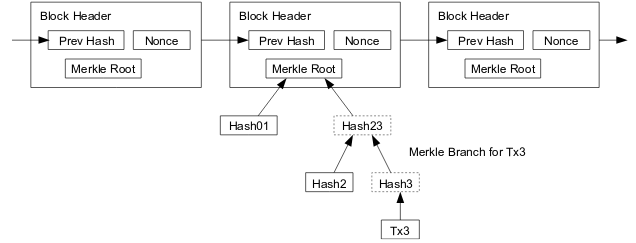
\includegraphics[scale=0.4]{blockchain}
	\caption{Imagem tirada do whitepaper do Bitcoin.}
	\label{fig:blockchain}
\end{figure}

\section{Contratos inteligentes}

Já no surgimento da blockchain descrito no protocolo do Bitcoin, havia espaço para 
criação de \textit{scripts} nas transações. Entretanto, estes \textit{scripts} foram concebidos
para serem simples, com a ideia de não sobrecarregar a rede com a execução de códigos
complexos. Um exemplo de \textit{script} trivial seria o congelamento de fundos até
certa data futura. Como não são  permitido \textit{loops} em sua estrutura, isto impacta
na não Turing completude da linguagem de \textit{script}.\cite{nakamoto2012bitcoin}

Almejando-se ter \textit{scripts} mais potentes, foi criado o conceito de contratos
inteligentes, que são Turing-completos e ainda guardam o estado atual do sistema.
\cite{ethereum}

Desta forma, é possível criar aplicações que rodam de forma descentralizada e que podem
ter seu estado atual verificado por qualquer participante do sistema em qualquer
momento além de garantir as propriedades da blockchain.

\bibliographystyle{abnt-alf}
\bibliography{ref}

\end{document}
